\label{chap:resultados}
Similar ao Seção \ref{sec:metastream}, os resultados são divididos em fases \textit{offline} e \textit{online}. Na avaliação \textit{offline}, nós analisamos o meta-classificador a respeito do quão bem ele consegue discriminar as classes no nível meta. Na avaliação \textit{online}, nós medimos os ganhos a respeito do desempenho preditivo no nível base quando aplicado a recomendação de algoritmos pelo meta-classificador. Os experimentos foram executados em um cluster com dois processadores Intel Xeon Silver 4114 de 2,20GHz com 256 Gb de RAM. O sistema operacional desta máquina é o Debian 9.

\section{Analise \textit{offline}}

A Tabela \ref{tab:algo_dist} lista a distribuição de algoritmos (RF e SVM\footnote{Uma aproximação do SVM como descrito na seção metodologia.}) que apresentam o melhor desempenho para cada lote do fluxo de dados (\textit{Electricity}, \textit{CoverType}, \textit{PowerSupply}, \textit{HyperPlane}, \textit{Agrawal} e \textit{RandomRBF}). Na perspectiva de MtA, essa tabela apresenta a distribuição de classes dos meta-exemplos para os meta-dados \textit{offline}.

\begin{table}[ht]
\caption{Distribuição de algoritmos nos meta-dados por problema de fluxo de dados.}
\label{tab:algo_dist}
\centering
\begin{tabular}{c|c|c} \hline
    Conjunto de Dados & SVM   & RF    \\ \hline
    Electricity       & 0.752 & 0.248 \\
    CoverType         & 0.718 & 0.282 \\
    PowerSupply       & 0.535 & 0.465 \\ \hline
    HyperPlane        & 0.792 & 0.207 \\
    Agrawal           & 0.785 & 0.215 \\
    RandomRBF         & 0.535 & 0.465 \\
\end{tabular}
\end{table}

Em termos gerais o algoritmo SVM apresentou melhor desempenho em relação ao RF para todos
os conjuntos de fluxos de dados. Para os conjuntos \textit{PowerSupply} e \textit{RandomRBF} o desempenho foi quase balanceado entre eles. Já nos outros conjuntos a distribuição está bem
desbalanceada para o SVM, logo, treinamos o meta-classificador para que lidasse com esse
desbalanceamento,  ajustando a função custo em razão da proporção das classes. 

Nós então estimamos o desempenho preditivo do meta-classificador usando um validação cruzada para series temporais, como descrito em \cite{hyndman2018forecasting}, para os dados iniciais. O modelo é inicialmente induzido na primeira janela de $\omega_m=300$ exemplos de treino e prevê as classes dos próximos $\eta_m=10$ exemplos de teste, então ambas as janelas deslizam 1 exemplo para a próxima avaliação. A Tabela \ref{tab:offmetrics} apresenta a média e o desvio padrão para essas métricas. Ganhos da meta-recomendação advém da recomendação não trivial dos algoritmos. Dado que o método Padrão representa um Kappa igual a zero, $Kappa=0$, $Kappa > 0$ representa um ganho preditivo.


\begin{table}[ht]
\caption{Desempenho preditivo do meta-classificador na fase \textit{offline}.}
\label{tab:offmetrics}
\centering
\begin{tabular}{c|c|c|c}\hline
    Fluxo   & Kappa           & M. Geométrica   & Acurácia        \\ \hline
Electricity & 0.095$\pm$0.176 & 0.366$\pm$0.207 & 0.610$\pm$0.152 \\
CoverType   & 0.018$\pm$0.215 & 0.329$\pm$0.232 & 0.517$\pm$0.147 \\
PowerSupply & 0.251$\pm$0.282 & 0.520$\pm$0.252 & 0.611$\pm$0.188 \\ \hline
HyperPlane  & 0.118$\pm$0.326 & 0.120$\pm$0.325 & 0.841$\pm$0.080 \\
Agrawal     & 0.007$\pm$0.138 & 0.046$\pm$0.164 & 0.780$\pm$0.078 \\
RandomRBF   & 0.120$\pm$0.239 & 0.416$\pm$0.262 & 0.571$\pm$0.115 \\
\end{tabular}
\end{table}

A Tabela \ref{tab:offmetrics} apresenta o desempenho preditivo da fase \textit{offline} avaliadas por três medidas distintas na configuração de janela deslizante. A acurácia é estimada sobre $\eta_m=10$, que é comparável a distribuição dos meta-dados da Tabela \ref{tab:algo_dist}. Para as medidas Kappa e Média Geométrica, nós removemos os exemplos em $\eta_m$ onde não tiveram diferença significativa entre os desempenhos dos algoritmos no nível base, isto é, nós computamos essas medidas para os exemplos base onde $|\text{Acc}(\text{RF})-\text{Acc}(\text{SVM})| > 0.1$. Essa abordagem foi aplicada com o objetivo de produzir uma mensuração mais apropriada do meta-classificador, pois onde não há uma diferença clara entre o desempenho dos modelos, qualquer um deles pode ser escolhido sem perdas.

Para todos os conjuntos, a medida Kappa é pelo menos levemente positiva, mostrando que o recomendador consegue selecionar o algoritmo correto quando há uma diferença significativa no desempenho preditivo entre eles, superando o método padrão. Acurácia é próxima da distribuição da classe majoritária, mas posteriormente iremos argumentar que grande parte dos exemplos não há diferença clara e alguns exemplos apresentam um ganho melhor de predição que outros, o que no nível base reflete em uma diferença significativa.

Para avaliar o quanto os meta-atributos contribuem ao sistema de recomendação, a Figura \ref{fig:fi} mostra os $5$ melhores meta-atributos, para cada conjunto, selecionado pelo algoritmo LightGBM. Nessa figura, o eixo $x$ representa a importância dos atributos dos meta-modelos dados pelo LightGBM, e o eixo $y$ mostra esses meta-atributos. A grande maioria dos meta-atributos selecionados por nós para dividir os dados foram do grupo de landmarking, seguido por baseado em modelo e estatístico. Esses grupos tem o maior grau informativo e discriminativo de acordo com a literatura \cite{Rivolli2018}.

\begin{figure}[ht]
    \centering
    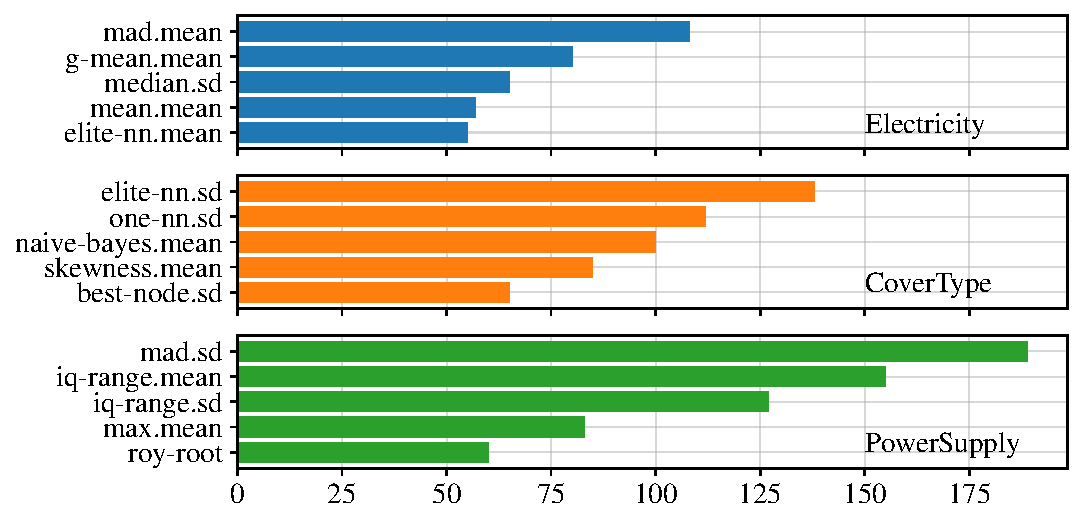
\includegraphics[width=0.8\linewidth]{general_fi}
    \caption{Importância dos atributos para o meta-algoritmo nos dados \textit{offline}.}
    \label{fig:fi}
\end{figure}


\section{Analise \textit{online}}

Na fase \textit{online}, nós avaliamos o meta-classificador (LightGBM) usando uma estratégia incremental e não incremental. Na avaliação passada, nós treinamos o meta-classificador usando o procedimento descrito na Seção \ref{subsec:online}. Quando novos meta-atributos estão disponíveis, o meta-classificador e retreinado do zero, e isto pode levar a um modelo completamente independente do modelo passado. Na estratégia \textit{online}, o LightGBM atualiza o modelo anterior, adaptando as árvores de decisão para se ajustar aos meta-exemplos da janela mais recente, atualizando assim os pesos de cada nó, mas sem substitui-los. A Tabela \ref{tab:onmetrics} apresenta esses resultados.


\begin{table}[ht]
\caption{Desempenho preditivo do meta-classificador na fase \textit{online}.}
\label{tab:onmetrics}
\centering
\begin{tabular}{r|l|c|c|c} \hline
Dataset     &  Estratégia    & Kappa & M. Geométrica & Acurácia \\ \hline
\multirow{2}{*}{Electricity} &  Non-Incremental      & 0.027 & 0.462  & 0.558    \\
            &  Incremental & 0.039 & 0.422  & 0.457    \\ \hline
\multirow{2}{*}{CoverType}   &  Non-Incremental       & 0.114 & 0.461  & 0.694    \\
            &  Incremental & -0.009 & 0.405  & 0.631    \\ \hline
\multirow{2}{*}{PowerSupply} &  Non-Incremental      & 0.092 & 0.502  & 0.607    \\
            &  Incremental & 0.074 & 0.541  & 0.539 \\ \hline
\multirow{2}{*}{HyperPlane}   &  Non-Incremental       & 0.014 & 0.265  & 0.747    \\
            &  Incremental & 0.020 & 0.283  & 0.745    \\ \hline
\multirow{2}{*}{Agrawal}   &  Non-Incremental       & 0.010 & 0.198  & 0.794    \\
            &  Incremental & -0.041 & 0.327  & 0.700    \\ \hline
\multirow{2}{*}{RandomRBF}   &  Non-Incremental       & -0.031 & 0.484  & 0.484    \\
            &  Incremental & 0.004 & 0.486  & 0.501
\end{tabular}
\end{table}

Embora a Tabela \ref{tab:onmetrics} apresente valores para Kappa relativamente baixos, nós notamos que esse valor é positivo para quase todas as combinações de conjunto-estratégia. Esses resultados indicam que o meta-classificador consegue selecionar o algoritmo mais apropriado comparado com a classe majoritária. Esse resultado é mais evidente para o conjunto \textit{PowerSupply}, que apresenta a melhor média geométrica e Kappa. Essa consistência refletirá posteriormente nos ganhos acumulados para esse conjunto. A estratégia incremental apresenta melhores desempenhos em relação a não incremental para os conjuntos \textit{Electricity}, \textit{HyperPlane} e \textit{RandomRBF}, para os outros conjuntos o incremental desempenhou pior para essas métricas.

Figuras \ref{fig:cumsum_elec2}-\ref{fig:cumsum_powersupply} mostram o ganho cumulativo, que é a diferença entre a acurácia do algoritmo recomendado e a acurácia do método Padrão. A região preenchida é a soma aculumada dessas diferenças de desempenho ao longo do tempo enquanto as cores laranja e azul representam as estratégias incrementais e não incrementais, respectivamente. Cada ponto preto representa o ganho de escore no tempo $t$.

\begin{figure}[!t]
    \centering
    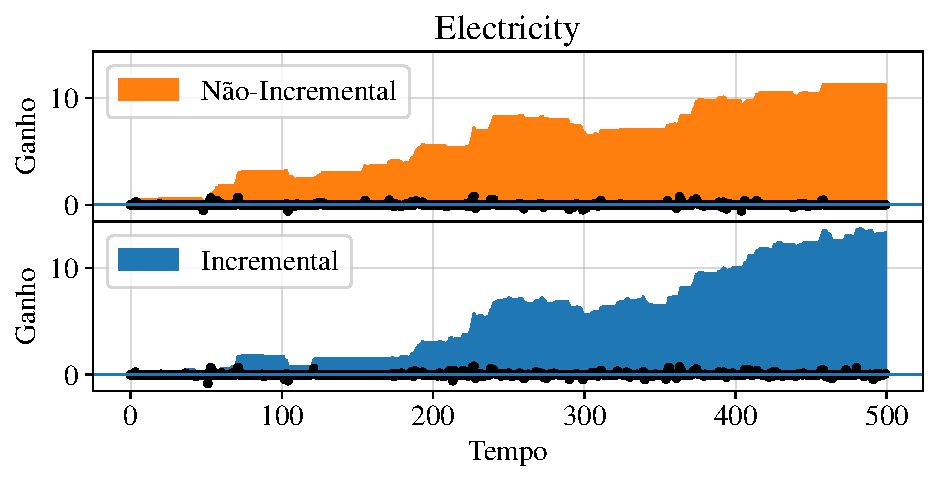
\includegraphics[width=0.8\linewidth]{elec2_cumsum}
    \caption{Ganho cumulativo de acurácia ao longo do tempo para o conjunto Electricity.}
    \label{fig:cumsum_elec2}
\end{figure}

\begin{figure}[!t]
    \centering
    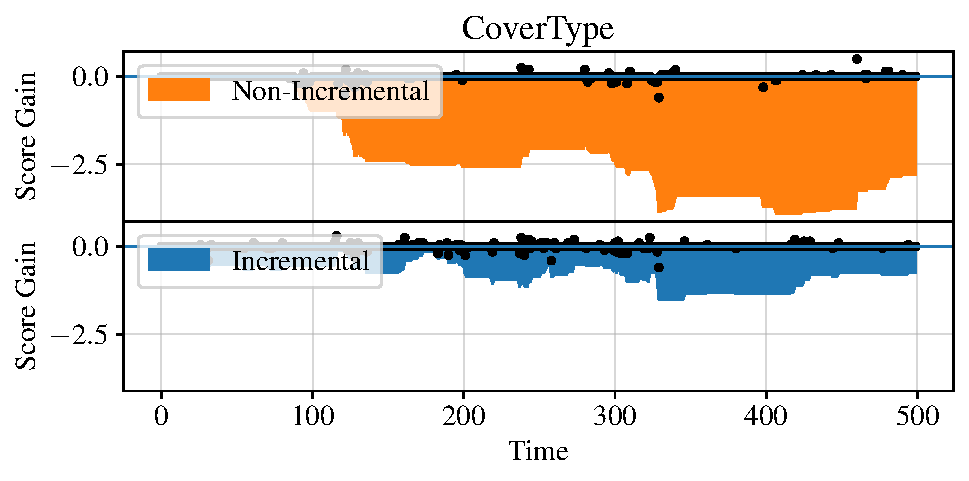
\includegraphics[width=0.8\linewidth]{covtype_cumsum}
    \caption{Ganho cumulativo de acurácia ao longo do tempo para o conjunto CoverType.}
    \label{fig:cumsum_covtype}
\end{figure}

\begin{figure}[!t]
    \centering
    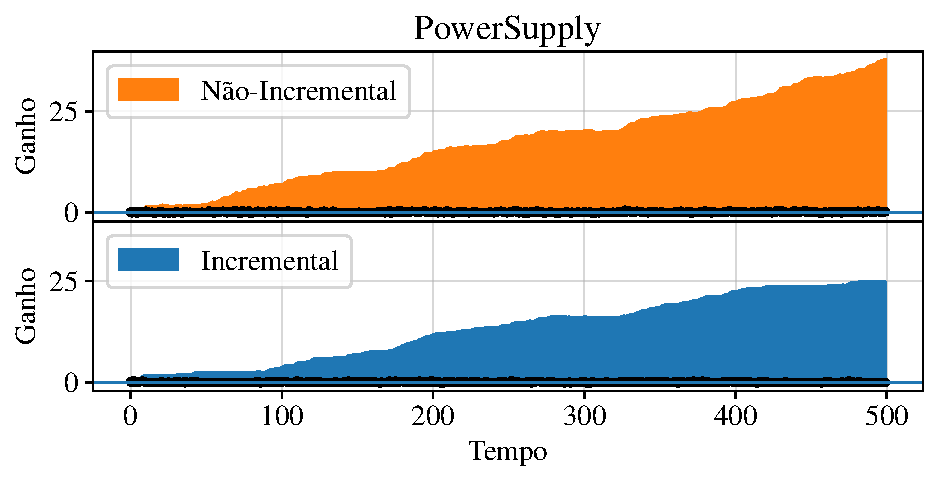
\includegraphics[width=0.8\linewidth]{powersupply_cumsum}
    \caption{Ganho cumulativo de acurácia ao longo do tempo para o conjunto PowerSupply.}
    \label{fig:cumsum_powersupply}
\end{figure}

Nessas figuras, nós observamos um ganho positivo para o \textit{Electricity} e o \textit{PowerSupply}. Já para o conjunto \textit{CoverType}, para essas configurações, o MetaStream falhou em selecionar efetivamente o melhor algoritmo, representado pela perda desempenho, escore negativo. Em termos gerais há um empate entre as estratégias para os conjuntos de dados reais, nas próximas figuras são apresentados os conjuntos sintéticos.

\begin{figure}[!t]
    \centering
    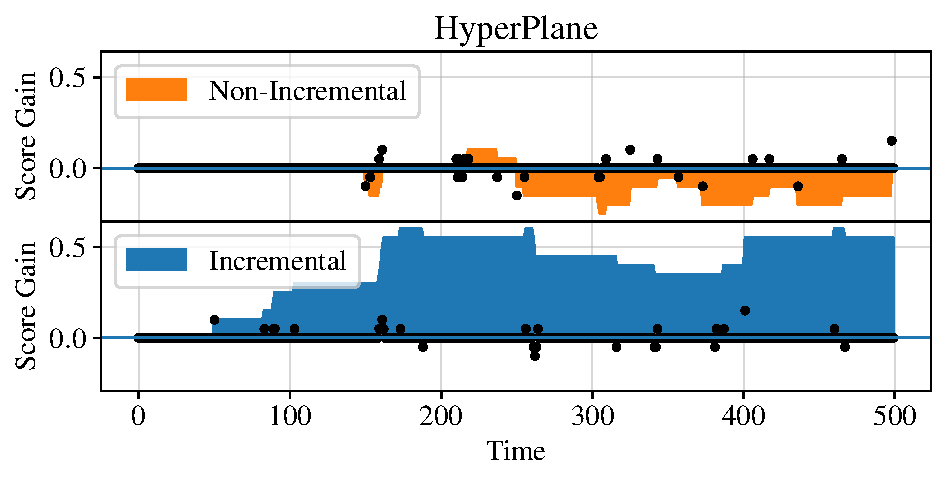
\includegraphics[width=0.8\linewidth]{hyper_cumsum}
    \caption{Ganho cumulativo de acurácia ao longo do tempo para o conjunto HyperPlane.}
    \label{fig:cumsum_hyper}
\end{figure}

O conjunto de dados sintético \textit{HyperPlane} apresentou um ganho inconsistente para o método não incremental e um ganho ligeiramente positivo para o método incremental.

\begin{figure}[!t]
    \centering
    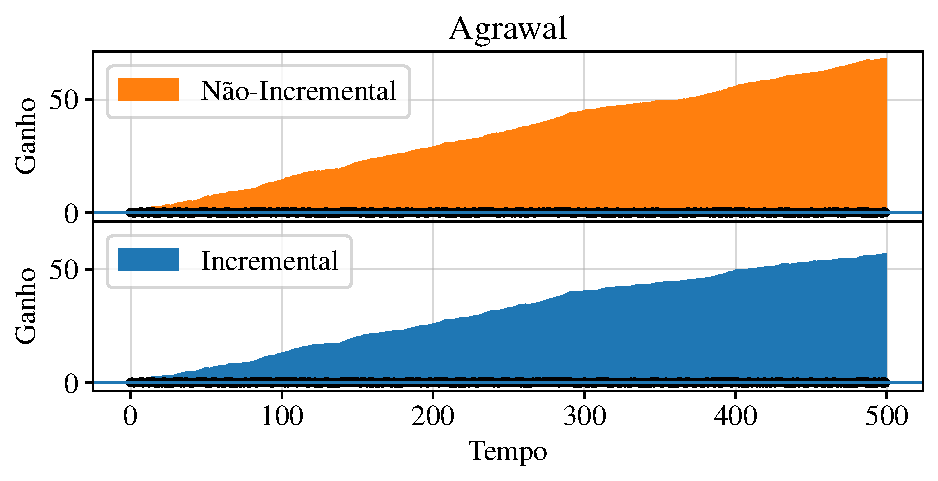
\includegraphics[width=0.8\linewidth]{agrawal_cumsum}
    \caption{Ganho cumulativo de acurácia ao longo do tempo para o conjunto Agrawal.}
    \label{fig:cumsum_agrawal}
\end{figure}

Com o Agrawal \textit{HyperPlane} tivemos um resultado bem diferente, o framework conseguiu obter ganhos consideráveis para ambos os métodos, tendo em média ganho de mais de 0.1 de acurácia por recomendação.

\begin{figure}[!t]
    \centering
    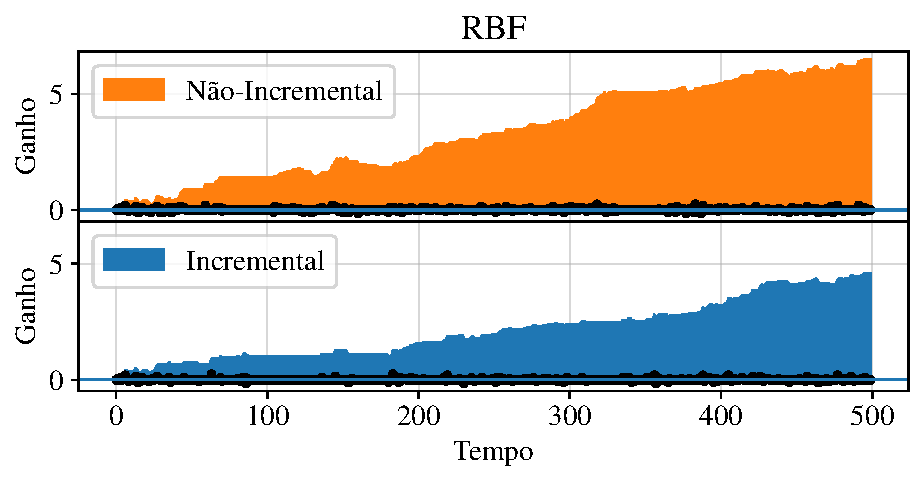
\includegraphics[width=0.8\linewidth]{rbf_cumsum}
    \caption{Ganho cumulativo de acurácia ao longo do tempo para o conjunto RandomRBF.}
    \label{fig:cumsum_rbf}
\end{figure}

Por fim, o conjunto \textit{RandomRBF} apresentou ganhos positivos, mas mais significativamente para o método não incremental. Para os conjuntos sintéticos, podemos ver um ganho para todas as recomendações pelo algoritmo incremental, sendo no caso do \textit{HyperPlane} ligeiramente negativo para o algoritmo não incremental.

Nas Figuras \ref{fig:scorecross_elec2}, \ref{fig:scorecross_covtype} e \ref{fig:scorecross_powersupply} as acurácias para o Padrão são dispostas contra as acurácias do Recomendado em um histograma bi-dimensional por mapa de calor. Logo, cada quadrado no mapa de calor representa a acurácia do algoritmo recomendado pelo método Padrão (eixo $x$) e pelo meta-classificador (eixo $y$) para a mesma janela. A intensidade da cor, como mostrado na barra de cores, representa o numero de pontos naquela posição. Os pontos da diagonal, onde o algoritmo recomendado e o padrão tiveram a mesma acurácia, foram removidos e coloridos de branco, para enfatizar apenas os pontos de ganhos e perdas do \textit{framework}. Se o classificador recomendado sempre for pior que o Padrão, isto é, recomendar a classe minoritária quando esta não é melhor que a majoritária, então todos os pontos ficaram abaixo da diagonal. Similarmente, esse pontos estarão acima se efetivamente selecionar o algoritmo da classe minoritária quando esse for melhor que a majoritária.

\begin{figure}[!t]
    \centering
    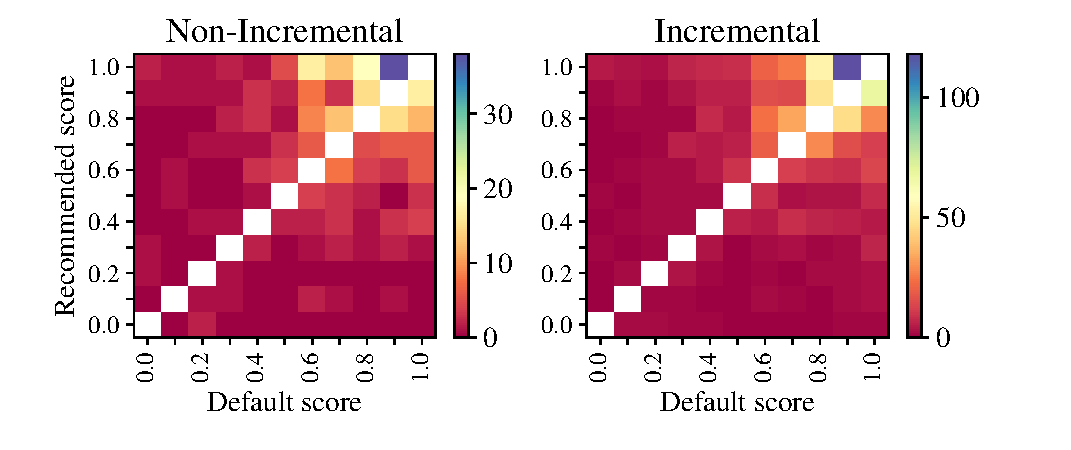
\includegraphics[width=0.8\linewidth]{elec2_score}
    \caption{Comparação entre o método recomendado e o padrão para o Electricity.}
    \label{fig:scorecross_elec2}
\end{figure}

Na Figura \ref{fig:scorecross_elec2}, é visível na região  superior direita do mapa de calor que o algoritmo incremental está recomendando a classe minoritária mais vezes que não-incremental, também o quadrado azul acima da diagonal branca tem mais pontos (100+ comparado a 30+ no não-incremental), isso reflete os ganhos mostrados na Figura \ref{fig:cumsum_elec2}.

\begin{figure}[!t]
    \centering
    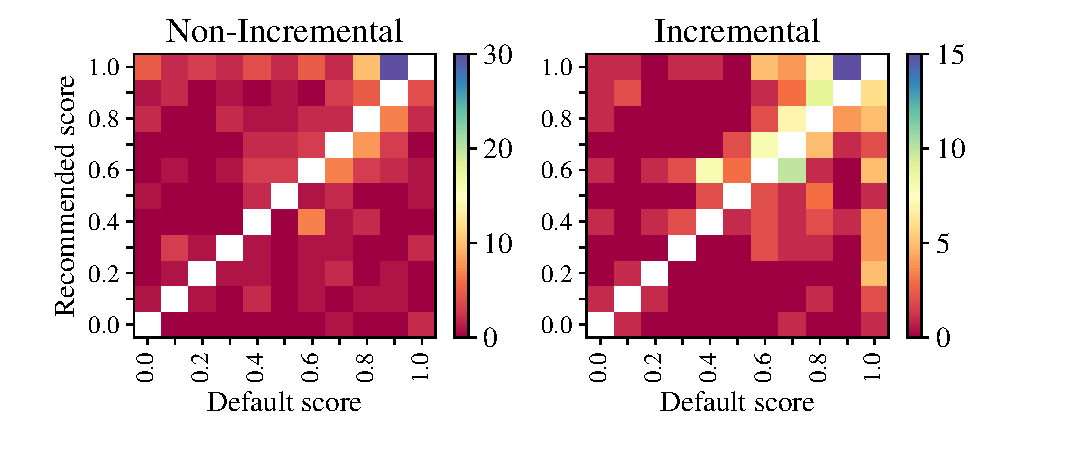
\includegraphics[width=0.8\linewidth]{covtype_score}
    \caption{Comparação entre o método recomendado e o padrão para o CoverType.}
    \label{fig:scorecross_covtype}
\end{figure}

Para o \textit{Covertype} (Figura \ref{fig:scorecross_covtype}), nós observamos um comportamento diferente, há um quadrado azul acima da diagonal para o gráfico não-incremental com uma grande quantidade de pontos e um quadrado verde claro abaixo da diagonal no incremental. Porém, a quantidade de pontos nessas regiões não é significativa em razão aos mil pontos do ganho acumulado e podemos ver que para esse conjunto de dados e a respectiva configuração do experimento o Metastream falha em recomendar o melhor algoritmo \ref{fig:cumsum_covtype}.

\begin{figure}[!t]
    \centering
    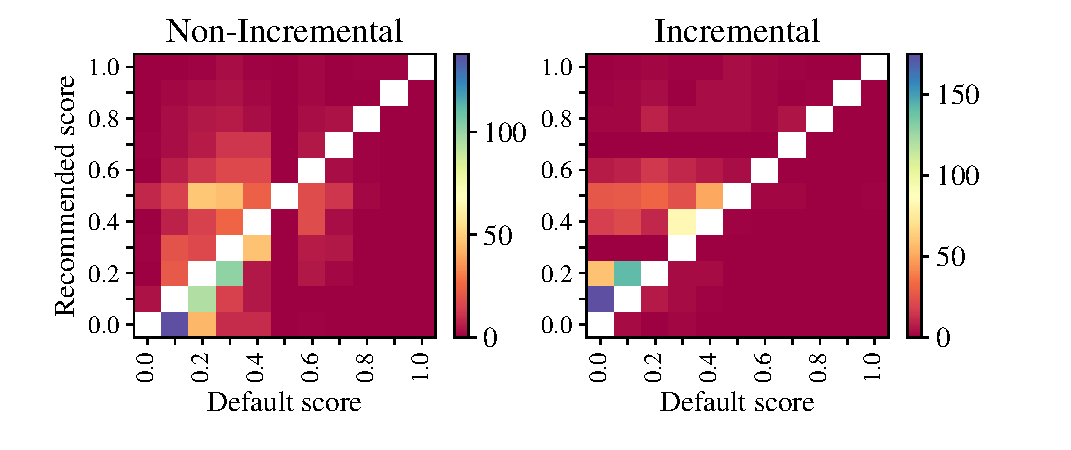
\includegraphics[width=0.8\linewidth]{powersupply_score}
    \caption{Comparação entre o método recomendado e o padrão para o PowerSupply.}
    \label{fig:scorecross_powersupply}
\end{figure}

O \textit{PowerSupply}, que tem 24 classes, é um dos mais difíceis de classificar, dado que todos os pontos tem acurácia abaixo de 0.8 como mostrado na Figura \ref{fig:scorecross_powersupply}. Entretanto, no nível meta, o recomendador teve grande sucesso em discriminar os algoritmos, tendo em vista que é um meta-dado balanceado, isso se refletiu no maior ganho por recomendação entre os conjuntos de dados reais, confirmado pela Figura  \ref{fig:cumsum_powersupply}.

\begin{figure}[!t]
    \centering
    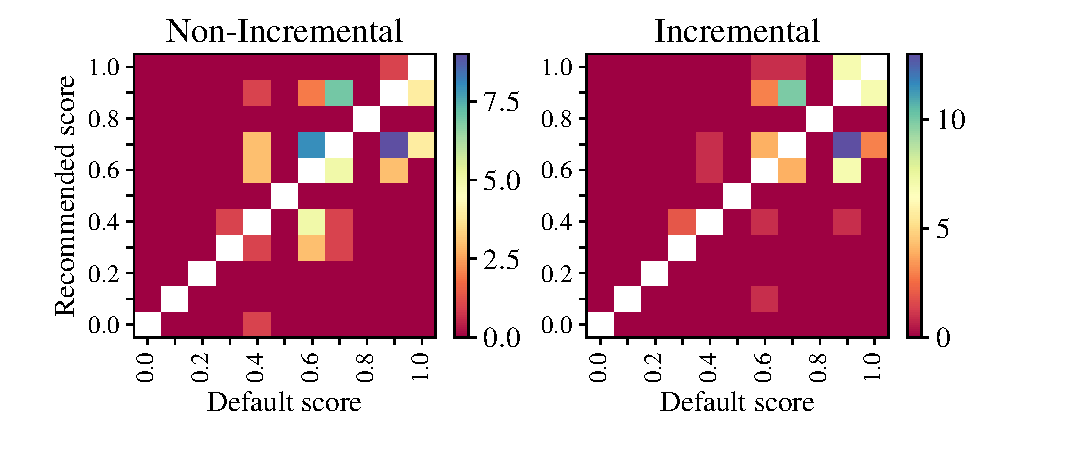
\includegraphics[width=0.8\linewidth]{hyper_score}
    \caption{Comparação entre o método recomendado e o padrão para o HyperPlane.}
    \label{fig:scorecross_hyper}
\end{figure}

No histograma da Figura \ref{fig:scorecross_hyper}, podemos ver que ambos os métodos fizeram poucas recomendações para esse conjunto de dados, sendo a meta-base composta por quase 80\% de exemplos da classe majoritária o meta-classificador não consegue aprender muito bem nessa configuração.

\begin{figure}[!t]
    \centering
    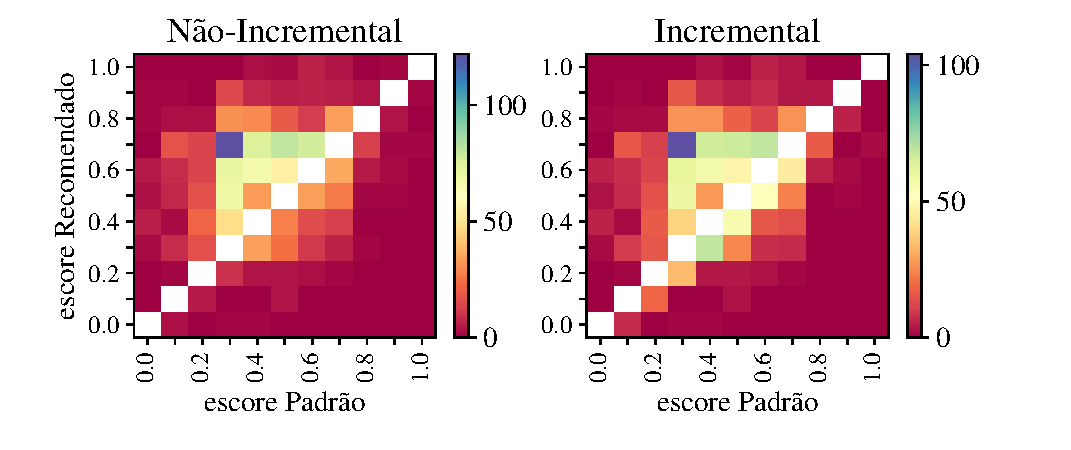
\includegraphics[width=0.8\linewidth]{agrawal_score}
    \caption{Comparação entre o método recomendado e o padrão para o Agrawal.}
    \label{fig:scorecross_agrawal}
\end{figure}

Para o conjunto \textit{Agrawal} temos um gráfico bem assimétrico para cima da diagonal, tendo regiões com mais de 100 pontos, resultando assim em um ganho significativo ao longo do tempo.

\begin{figure}[!t]
    \centering
    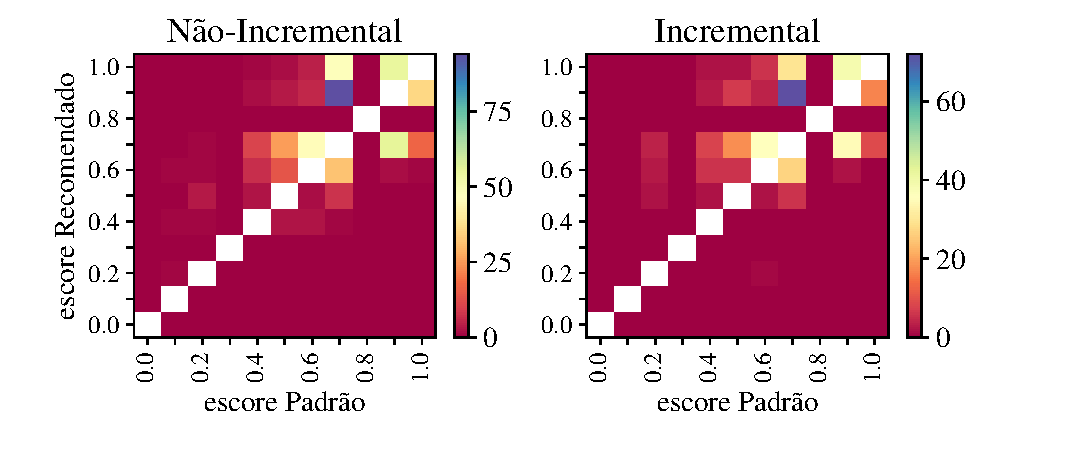
\includegraphics[width=0.8\linewidth]{rbf_score}
    \caption{Comparação entre o método recomendado e o padrão para o RandomRBF.}
    \label{fig:scorecross_rbf}
\end{figure}

Já o conjunto \textit{RandomRBF} tiveram menos pontos acima da diagonal mas ainda sim os pontos de máximo se localizam acima da diagonal, tendo um ganho consistentemente positivo.

\begin{figure}[!t]
    \centering
    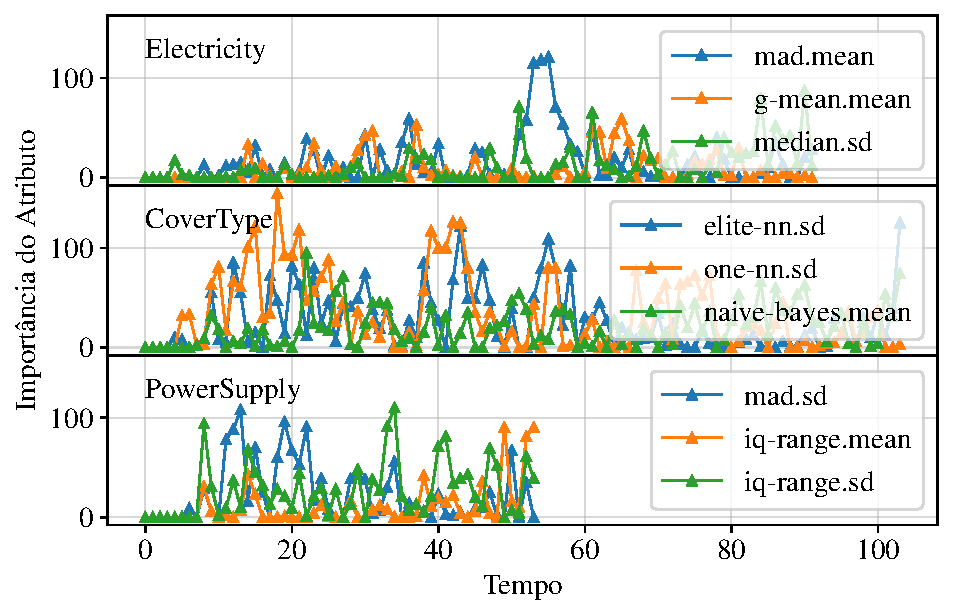
\includegraphics[width=0.8\linewidth]{general_timefi}
    \caption{Variação na importância dos atributos ao longo do tempo para três meta-atributos.}
    \label{fig:fi_time}
\end{figure}

A importância dos atributos da estratégia incremental é dada pela Figura \ref{fig:fi}, dado que o método incremental mantém os mesmos atributos dos nós do treinamento nos dados \textit{offline}, alterando apenas seus valores. Já no caso do método não-incremental uma nova árvore é construída do zero, podendo então variar a importância dos atributos. Como apresentado na Figura \ref{fig:fi_time}, há uma variação significativa dessa importância para cada janela de treinamento. Acreditamos que fixar a importância dos atributos acarreta em uma forma de regularização sobre o algoritmo. Entretanto, alternativamente, mudanças de conceito podem ocorrer a nível meta, sendo então possivelmente benéfico permitir que a escolha da árvore seja mais flexível.